
\chapter{Grundlagen}

Der Begriff einer Abbildung ist uns schon öfter untergekommen. Eine Funktion ist eine Abbildung, die zwei Mengen (hier $X$ und $Y$) in Beziehung setzt:

\[ f: X \longrightarrow Y \]
$f$ ordnet jedem Element $x\in X$ ein Element $y\in Y$ zu, indem
\[f(x) =y\]
gilt. Die Umkehrung gibt es allgemein nicht, aber wenn sie existiert, so wird sie als $f^{-1}$ bezeichnet und es gilt:
\[ f^{-1}(y) =x\]

\begin{definition}
Der Begriff \textsl{Funktion} ist identisch mit dem Begriff Abbildung. 
\end{definition}


\section{Polynome}

Wir hatten in Kapitel \ref{chap:poly} Polynome bereits kennengelernt. Polynome -- wie wir sie hier betrachten -- sind Funktionen $p :\mathbb{R} \longrightarrow \mathbb{R}$. Wir betrachten also hier grundsätzlich reelle Polynome. Wenn wir Polynome auf dem komplexen Zahlen betrachten, wird dies extra angemerkt.

Im allgemeinen betrachten wir Polynome vom Rang $n$, das heißt Funktionen der Form
\[
p(x) = \sum_{i=0}^{n} a_i \cdot x^i
\]
wobei der Wert des Parameters $x$ in keiner Weise festgelegt wird. Wir betrachten also das Polynom in seiner Gesamtheit, ohne Einschränkung auf einen bestimmten Wert $x$. Mit der Abbildung 
\[
\phi(p,x) = \phi\left( \sum_{i=0}^{n} a_i \cdot x^i \right) = \begin{pmatrix}
a_0\\ a_1 \\ a_2 \\ \vdots \\ a_n
\end{pmatrix}
\]
identifizieren wir jedes Polynom mit einem Vektor aus dem $\mathbb{R}^{n+1}$. Für jeden beliebigen Vektor $v\in \mathbb{R}^{n+1}$ ist 
\[ 
\phi^{-1}(v,x) = \sum_{i=0}^{n} v_i \cdot x^i
\]
Daraus folgt, dass die Abbildung $\phi$ die Vektorraumstruktur des $\mathbb{R}^{n+1}$ auf den Raum aller Polynome mit Grad $\le n$ abbildet und somit diese ebenfalls einen Vektorraum bilden. Dieser wird 
\[P_n =\left\lbrace p \ \middle\vert \  p(x) = \sum_{i=0}^{n} a_i \cdot x^i, \ (a_i)_i \in \mathbb{R}^{n+1} \right\rbrace  \]
genannt. Zur Vertiefung seien die Anforderungen A1-A4 und M1-M4 aus Kapitel \ref{vectorspace} für $P_n$ nachgewiesen.


\subsection{Ableitung von Polynomen}

Der Begriff der Abteilung von Funktionen wird später erst formal eingeführt. Da die Ableitung für Polynome sehr einfach zu bestimmen ist, wird der Begriff hier vorab für Polynome definiert und für die Details sei auf Kapitel \ref{chap:diff} verwiesen.

Es sei $v\in \mathbb{R}^{n+1}$ die Repräsentation im reellen Vektorraum des Polynoms $p\in P_n$. Es sei die folgende Abbildung $D: \mathbb{R}^{n+1} \longrightarrow \mathbb{R}^{n} $ definiert:

\begin{equation}
D(v) = D(v_i)_{i=0,\dots,n} = (i\cdot v_i)_{i=1,\dots,n}
= \begin{pmatrix}
1\cdot v_1 \\ 2\cdot v_2 \\ 3\cdot v_3 \\ \vdots \\ n\cdot v_n
\end{pmatrix}
\end{equation}

$D$ ist mehrfach anwendbar:
\[
D^2(v) = D(D(v)) = \begin{pmatrix}
1\cdot 2\cdot v_2 \\
2\cdot 3\cdot v_3 \\
\vdots \\
(n-1)\cdot n \cdot v_n
\end{pmatrix} \in \mathbb{R}^{n-1}
\]
usw. Aufgrund der Existenz der Umkehrung der Abbildung $\phi$ gibt es Polynome $D(p)$ mit 
\[
D(p(x)) = \sum_{i=1}^{n} i\cdot v_i \cdot x^{i-1}
\]
$D(p)$ wird die \textsl{erste Ableitung} von $p$ genannt, und
\[
D^2(p(x)) = \sum_{i=2}^{n} (i-1)\cdot i\cdot v_i \cdot x^{i-2}
\]
wird \textsl{zweite Ableitung} von $p$ genannt, usw.

Diese recht abstrakte Definition der Ableitungen ist zwar unüblich, hat aber den Vorteil, dass die Ableitung hier als einfache Abbildung auf einem Vektorraum dargestellt werden kann. 

Beispiel: Gegeben sei das Polynom 

\[
p(x) = x^3 + 2x^2 + 3x + 4
\]
Die erste Ableitung ist:
\[
D(p(x)) = 1\cdot 3\cdot x^2 + 2\cdot 2\cdot x + 1\cdot 3 = 3x^2 + 4x +3
\]
Die zweite Ableitung ist:
\[
D^2(p(x)) = D(3x^2 + 4x+3) = 2\cdot 3 x + 1\cdot 4 = 6x +4
\]
Was haben nun $D(p)$ und $D^2(p)$ mit $p$ zu tun? Das erschließt sich nicht einfach aus der Definition von $D$, aber wie wir im Kapitel über die Differentialrechnung sehen werden, ist $D(p)$ gerade die Funktion, deren Wert der Steigung von $p$ entspricht, wie $D^2(p)$ diejenige Funktion ist, deren Wert der Steigung von $D(p)$ entspricht. Wenn also, wie in Abbildung \ref{fig:polydiff} dargestellt, $D^2(p) = 0$ ist, so hat $D(p)$ an genau dieser Stelle einen sogenannten \textsl{Extremwert}, das bedeutet, alle Funktionswerte von $D(p)$ in einer Umgebung um diese Nullstelle von $D^2(p)$ sind größer oder kleiner als $D(p)$.


\begin{figure}
\begin{center}
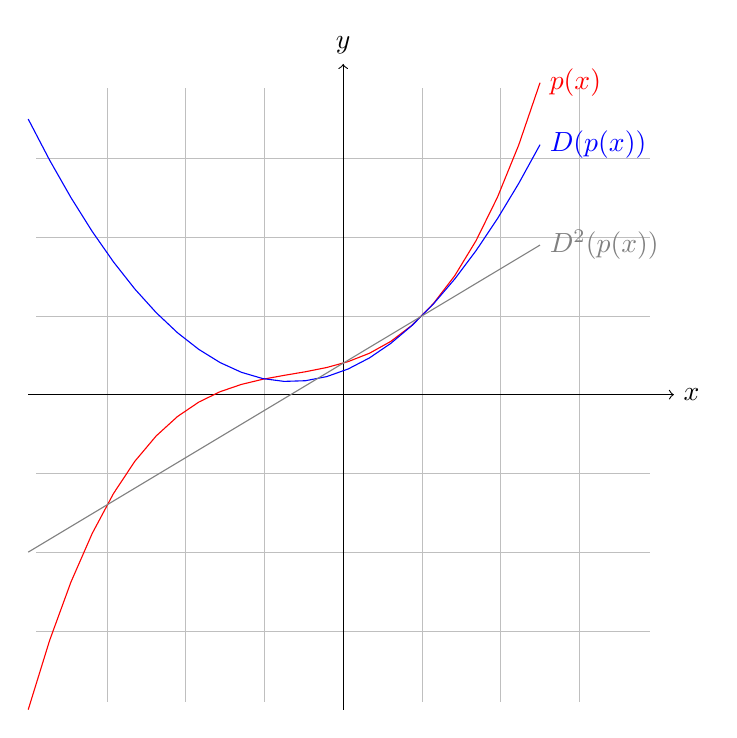
\begin{tikzpicture}[domain=-4:2.5]
\draw[very thin,color=lightgray] (-3.9,-3.9) grid (3.9,3.9);

\draw[->] (-4,0) -- (4.2,0) node[right] {$x$};
\draw[->] (0,-4) -- (0,4.2) node[above] {$y$};

\draw[color=red] plot (\x,\x*\x*\x/10+2*\x*\x/10+3*\x/10+4/10) node[right] {$p(x) $};
\draw[color=blue] plot (\x,3*\x*\x/10+4*\x/10+3/10) node[right] {$D(p(x)) $};
\draw[color=gray] plot (\x,6*\x/10+4/10) node[right] {$D^2(p(x)) $};
\end{tikzpicture}
\caption[Polynom mit Ableitungen]{Funktionen-Plot von $p(x)$, $D(p(x))$ und $D^2(p(x))$}
\label{fig:polydiff}
\end{center}
\end{figure}

\begin{definition}\index{Extremwert}
Gibt es für eine Funktion $f:\mathbb{R} \longrightarrow \mathbb{R}$ an einer Stelle $x_0 \in \mathbb{R}$ eine Umgebung $I = [x_0-\epsilon, x_0+\epsilon]$ mit $\epsilon>0 $, in der  für alle $z\in I$ entweder $f(z)\le f(x_0)$, oder $f(z)\ge f(x_0)$ gilt, so wird $x_0$ \textsl{Extremwert} genannt.
\end{definition}

\begin{definition}\index{lokales Maximum}
Gilt für $f,x_0,z,I$ wie oben, immer $f(z)\le f(x_0)$, so nennt man $x_0$ ein \textsl{lokales Maximum}.
\end{definition}

\begin{definition}\index{lokales Minimum}
Gilt für $f,x_0,z,I$ wie oben, immer $f(z)\ge f(x_0)$, so nennt man $x_0$ ein \textsl{lokales Minimum}.
\end{definition}

\begin{definition}\index{globales Maximum}
Gilt für $f,x_0$ wie oben, $f(z)\le f(x_0)$ für alle $z\in \mathbb{R}\backslash \{x_0\}$, so wird $x_0$ als \textsl{globales Maximum} bezeichnet.
\end{definition}

\begin{definition}\index{globales Minimum}
Gilt für $f,x_0$ wie oben, $f(z)\ge f(x_0)$ für alle $z\in \mathbb{R}\backslash \{x_0\}$, so wird $x_0$ als \textsl{globales Minimum} bezeichnet.
\end{definition}

\begin{definition}
Sei $p \in P_n$ und an $x_0$ sei $D^2(p(x_0))=0$. Gilt weiter $D^2(p(z))\ne 0$ für $z\in \mathbb{R}\backslash \{x_0\}$, so nennt man $x_0$ einen \textsl{Wendepunkt} von $p$.
\end{definition}

In Abbildung \ref{fig:polydiff} sieht man im Grafen von $p(x)$, wie dieser mit hoher Steigung von links unten in die Zeichnung hinein kommt. Dann flacht die Kurve ab, und ab $D^2(p(x))=0$ wird sie wieder steiler. Dies ist die Charakteristik eines Wendepunktes. Denn die Krümmung der Kurve des Grafen $p(x)$ wechselt von negativ (wird immer flacher), zu positiv (wird immer steiler).

Wie wir sehen, wird die Steigung von $p(x)$ direkt durch ihre erste und zweite Ableitung bestimmt.

\section{Kurvendiskussion}

Wie wir im vorherigen Abschnitt gesehen haben, sind die Nullstellen der ersten und zweiten Ableitung einer Funktion von besonderem Interesse, wenn uns die Form der Kurve interessiert. Eben diese ist Thema einer Kurvendiskussion.

\begin{definition}
Eine \textsl{Kurvendiskussion} ist eine Vorgehensweise, wie aus Informationen über Nullstellen einer Funktion, ihrer ersten und zweiten Ableitung, sowie einiger, ausgewählter Funktionswerte, genug Eigenschaften gefolgert werden können, um eine Funktion näherungsweise in einem Koordinatensystem zu zeichnen.
\end{definition}

Die folgenden Unterabschnitte verdeutlichen anhand eines Beispiels, wie eine Kurvendiskussion durchgeführt wird. Danach werden wir erst die Definitionen kennenlernen. 

Kurvendiskussionen sind heutzutage kaum noch notwendig. Üblicherweise nutzt man einen Computer zur Darstellung eines Funktionsgraphen. Ein "`raten"' seines Aussehens ist nicht notwendig. Da die Kurvendiskussion in Schulen aber noch seinen Platz hat, wird sie hier aufgezeigt. 

\subsection{Voraussetzungen}

Wir betrachten das Polynom $p(x) = x^3 -12x$. Es ist vom dritten Grad und seine Faktoren für das quadratische, sowie das konstante Monom sind 0. Wir berechnen

\begin{eqnarray*}
p(x) &=& x^3 -12x \\
D(p(x)) &=& 3x^2 -12 \\
D^2(p(x)) &=& 6x
\end{eqnarray*}


\subsection{Nullstellen von $p$}\label{sec:nsp}

Das Polynom $p$ ist vom dritten Grad, also gibt es drei Nullstellen. Die erste kann geraten werden, denn sie liegt genau im Null-Punkt. Es gilt
\begin{eqnarray*}
0 &=& x^3 -12x \qquad \vert \div x \\
0 &=& x^2 - 12 \qquad \vert +12 \\
12 &=& x^2 \qquad \vert \sqrt{.} \\
\pm \sqrt{12} &=& x
\end{eqnarray*}
Daraus folgt, dass $p$ folgende Nullstellen hat: $\{-\sqrt{12},0,+\sqrt{12}\}$.

\subsection{Nullstellen von $D(p)$}\label{sec:nsd1}

Die Nullstellen von $D(p(x))=3x^2-12$ sind ebenfalls einfach zu raten, aber wir berechnen sie hier der Vollständigkeit halber:
\begin{eqnarray*}
0 &=& 3x^2-12 \\
12 &=& 3x^2 \\
4 &=& x^2 \\
\pm \sqrt{4} &=& x \\
\pm 2 &=& x
\end{eqnarray*}
Die Nullstellen sind also $\{-2,2\}$. 

\subsection{Nullstellen von $D^2(p(x))$}\label{sec:nsd2}

Als lineare Funktion hat 
\[
D^2(p(x)) = 6x
\]
nur eine Nullstelle, und zwar bei $0$.

\subsection{Folgerungen}

Wir können aus dem vorherigen folgende Informationen folgern:

\begin{enumerate}
\item Aufgrund von Abschnitt \ref{sec:nsd2} hat $p$ einen Wendepunkt an der Stelle 0.
\item Sowie zwei Extremwerte an den Stellen $\{-2, +2\}$ aufgrund von Abschnitt \ref{sec:nsd1}.
\item $p$ nimmt an den Stellen $\{-2,2\}$ die Werte $\{16,-16\}$ an. 
\item $p$ hat Nullstellen in $\{-\sqrt{12},0,\sqrt{12}\}$.
\end{enumerate}




\subsection{Zusammenfassung im Graph}

\begin{figure}
\begin{center}
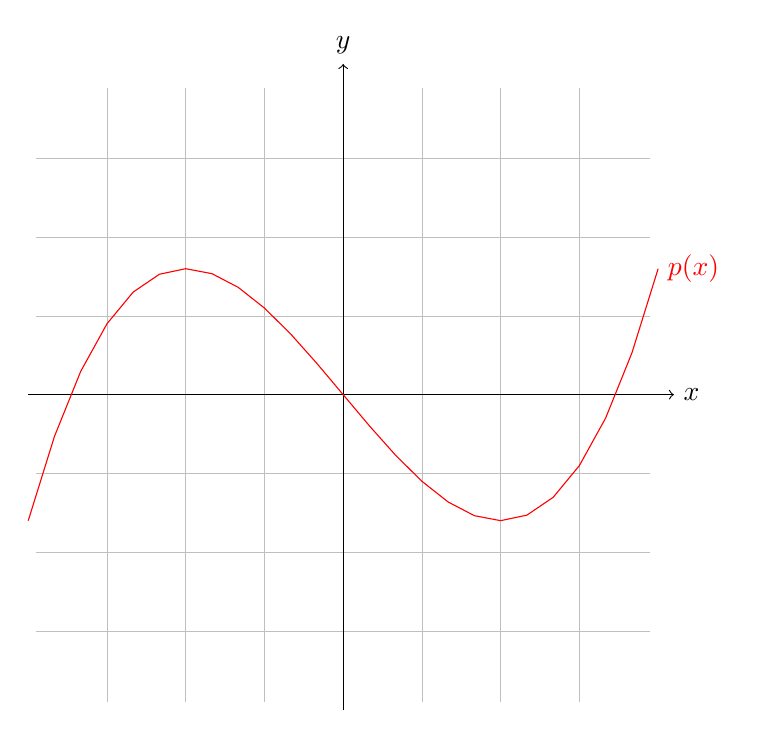
\begin{tikzpicture}[domain=-4:4]
\draw[very thin,color=lightgray] (-3.9,-3.9) grid (3.9,3.9);

\draw[->] (-4,0) -- (4.2,0) node[right] {$x$};
\draw[->] (0,-4) -- (0,4.2) node[above] {$y$};

\draw[color=red] plot (\x,\x*\x*\x/10-12*\x/10) node[right] {$p(x) $};
\end{tikzpicture}
\caption[Polynom zur Kurvendiskussion]{Verlauf von $p(x)$ anhand der Kurvendiskussion}
\label{fig:pkd}
\end{center}
\end{figure}


\begin{figure}
\begin{center}
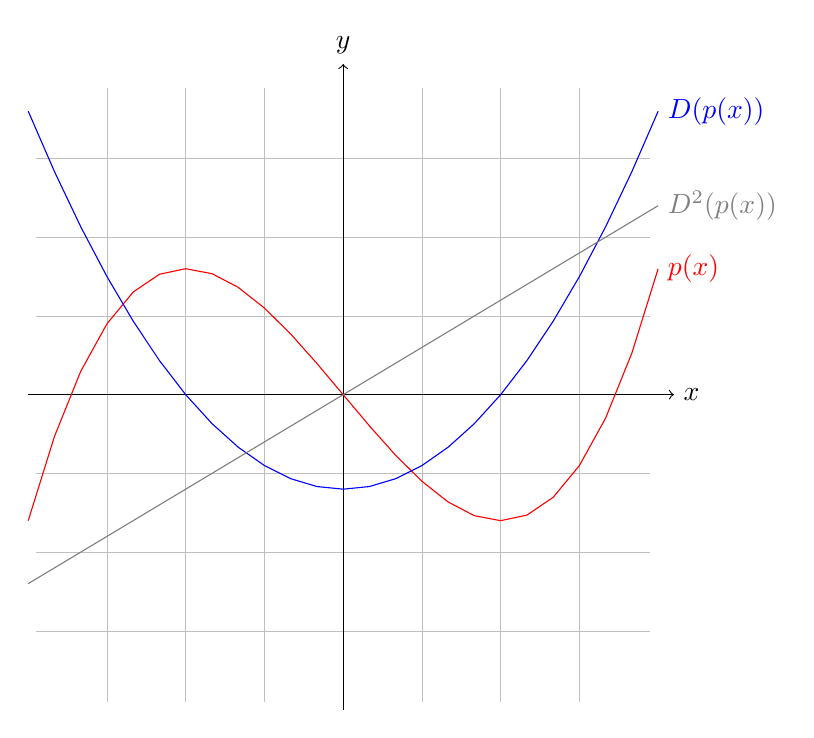
\begin{tikzpicture}[domain=-4:4]
\draw[very thin,color=lightgray] (-3.9,-3.9) grid (3.9,3.9);

\draw[->] (-4,0) -- (4.2,0) node[right] {$x$};
\draw[->] (0,-4) -- (0,4.2) node[above] {$y$};

\draw[color=red] plot (\x,\x*\x*\x/10-12*\x/10) node[right] {$p(x) $};
\draw[color=blue] plot (\x,3*\x*\x/10-12/10) node[right] {$D(p(x)) $};
\draw[color=gray] plot (\x,6*\x/10) node[right] {$D^2(p(x)) $};
\end{tikzpicture}
\caption[Vollständige Darstellung zur Kurvendiskussion]{Darstellung von $p(x)$, $D(p(x))$ und $D^2(p(x))$ zur Kurvendiskussion}
\label{fig:kdvoll}
\end{center}
\end{figure}

